\subsection{Moving average filter}
For at teste, hvorvidt moving average filteret overholder kravene, der er opstillet i \autoref{sec:mavg_krav} visualiseres forskellen mellem det ufiltrede signal samt det filtrede signal. Det optagede signal fra pilotforsøget \autoref{sec:pilotforsoeg} sendes til mikrokontrollen via en UART-forbindelse, som modtager den retunerede værdi. De sendte og returnerede værdier visualiseres i MATLAB. Resultatet heraf fremgår af \autoref{fig:mavg_test}. 

\begin{figure}[H]
	\centering
	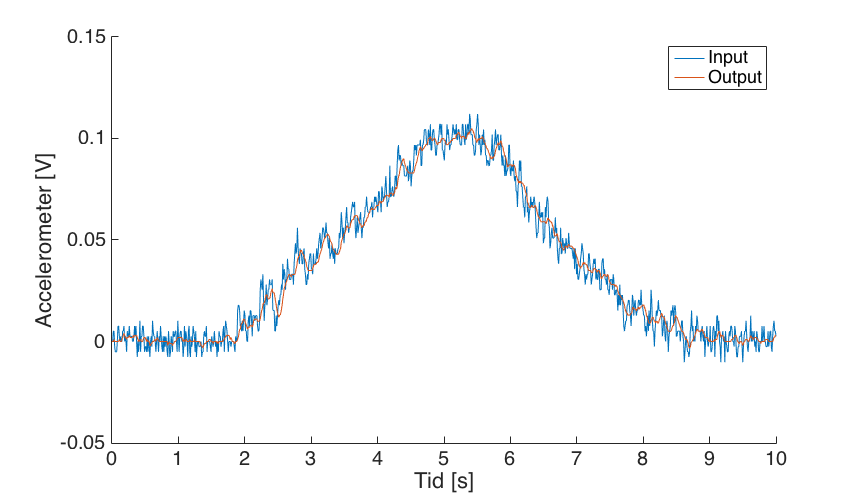
\includegraphics[width=1\textwidth]{figures/accelerometer_filter}
	\caption{Moving average filter programmeret i PSoC visualiseret i MATLAB}
	\label{fig:mavg_test}
\end{figure}

% Her skal der skrives hvad der kan ses af testen ift ændringerne i signalet. Dernæst vil filteret blive testet ift. det delay der forekommer. 

Da filteret kræver 10 samples for at retunere den første værdi testes det, hvorvidt dette stemmer overens med det forventede delay på $100~ms$. Dertil ses også om der forårsages yderligere delay af filteret. Til at måle behandlingstiden, programmeres en timer funktion i mikrokontrolleren, der retunerer behandlingstiden til MATLAB. Ud fra dette ses et delay på 34 sekunder og 60 milisekunder.

Ud fra ovenstående resultater vurderes det, at det filterede signal opfylder kravene for \autoref{sec:mavg_krav}. 